% Lecture Template for ME3001-001-Tristan Hill - Spring 2017 - Fall 2017
% 
% Mechanical Engineering Analysis with MATLAB
%
% Systems of Linear Equations - Lecture 4
%


% Document settings
\documentclass[11pt]{article}
\usepackage[margin=1in]{geometry}
\usepackage[pdftex]{graphicx}
\usepackage{multirow}
\usepackage{setspace}
\usepackage{hyperref}
\usepackage{color,soul}
\usepackage{fancyvrb}
\usepackage{framed}
\usepackage{wasysym}
\usepackage{multicol}
\usepackage{amssymb}

\pagestyle{plain}
\setlength\parindent{0pt}
\hypersetup{
    bookmarks=true,         % show bookmarks bar?
    unicode=false,          % non-Latin characters in Acrobat’s bookmarks
    pdftoolbar=true,        % show Acrobat’s toolbar?
    pdfmenubar=true,        % show Acrobat’s menu?
    pdffitwindow=false,     % window fit to page when opened
    pdfstartview={FitH},    % fits the width of the page to the window
    pdftitle={My title},    % title
    pdfauthor={Author},     % author
    pdfsubject={Subject},   % subject of the document
    pdfcreator={Creator},   % creator of the document
    pdfproducer={Producer}, % producer of the document
    pdfkeywords={keyword1} {key2} {key3}, % list of keywords
    pdfnewwindow=true,      % links in new window
    colorlinks=true,       % false: boxed links; true: colored links
    linkcolor=red,          % color of internal links (change box color with linkbordercolor)
    citecolor=green,        % color of links to bibliography
    filecolor=magenta,      % color of file links
    urlcolor=blue           % color of external links
}

% assignment number 
\newcommand{\NUM}{3} 
\newcommand{\VSpaceSize}{2mm} 
\newcommand{\HSpaceSize}{2mm} 

%\definecolor{mygray}{rgb}{.6, .6, .6}
%\definecolor{mypurple}{rgb}{0.6,0.1961,0.8}
\definecolor{mygreen}{rgb}{0.1333 ,  0.5451,    0.1333}
\definecolor{mypink}{rgb}{0.1333 ,  0.5451,    0.1333}
\setulcolor{red} 
\setstcolor{green} 
\sethlcolor{mygray} 

\definecolor{mygreen}{rgb}{0, .39, 0}

%\definecolor{dred}{#8B0000}
% [153,50,204] - dark orchid
\definecolor{mypurple}{rgb}{0.6,0.1961,0.8}
%[139,69,19] - saddle brown
\definecolor{mybrown}{rgb}{0.5451,0.2706,0.0745}

\definecolor{mygray}{rgb}{.6, .6, .6}

\setulcolor{red} 
\setstcolor{green} 
\sethlcolor{mygray} 

\newcommand{\VA}{\vspace{2mm}}
\newcommand{\VB}{\vspace{5mm}} 
\newcommand{\VC}{\vspace{30mm}} 
 
\newcommand{\R}{\color{red}}
\newcommand{\B}{\color{blue}}
\newcommand{\K}{\color{black}}
\newcommand{\G}{\color{mygreen}}
\newcommand{\PR}{\color{mypurple}}

\begin{document}

\textbf{ \LARGE ME 3001 Lecture - Systems of Linear Equations} \\\\
\textbf{ \LARGE Solution Existence and Potential Problems } \\


 \renewcommand\labelitemi{\textbullet}
 \renewcommand\labelitemii{\textendash}
 \renewcommand\labelitemiii{\textasteriskcentered}
 \renewcommand\labelitemiv{\textperiodcentered}

\Large
\begin{itemize}

\Large
\item \textbf{ Some problems cannot be solved with this type of technique!} \\	
\begin{itemize}
\item {\PR non-homogeneous} system is one in which ... \vspace{10mm}\\
\item most of the time the system will be {\PR non-homogeneous} \vspace{10mm}\\
\item a {\PR non-homogeneous} system has a {\B proper solution} if and only if ...\vspace{10mm}\\
	
	\scalebox{2}{$rank(A)=rank([A | b])=n$}

\newpage
\item {\bf Normal Case - 2 Equations - 2 Unknowns - 1 Solution} \\\\ 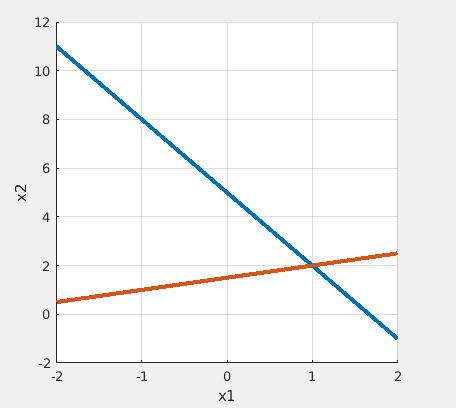
\includegraphics[scale=1]{lecture5_fig1.png} \\\\
\scalebox{2}{$3x_1+x_2=5$}\\\\
\scalebox{2}{$x_1-2x_2=-3$}

\newpage
\item {\bf Abnormal Case - 2 Equations - 2 Unknowns - $\infty$ Solutions} \\\\ 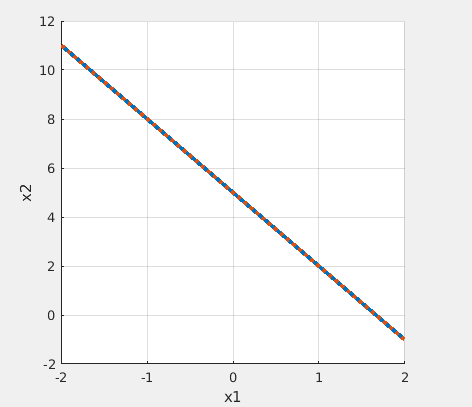
\includegraphics[scale=1]{lecture5_fig2.png} \\\\
\scalebox{2}{$3x_1+x_2=5$}\\\\
\scalebox{2}{$6x_1+2x_2=10$}

\newpage
\item {\bf Abnormal Case - 2 Equations - 2 Unknowns - 0 Solutions} \\\\ 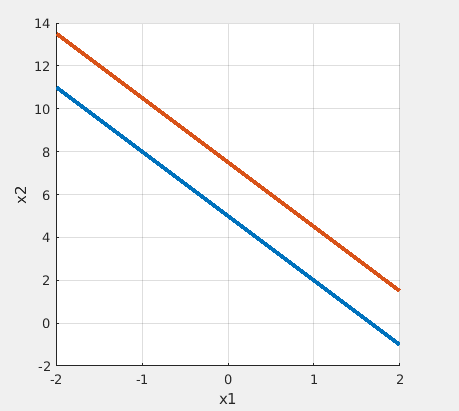
\includegraphics[scale=1]{lecture5_fig3.png} \\\\
\scalebox{2}{$3x_1+x_2=5$}\\\\
\scalebox{2}{$6x_1+2x_2=15$}

\newpage
\item {\bf Abnormal Case - 3 Equations - 2 Unknowns - 0 Solutions} \\\\ 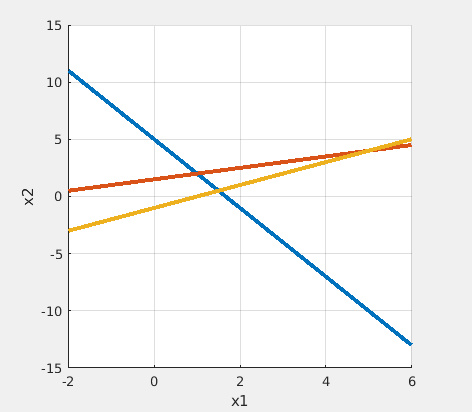
\includegraphics[scale=1]{lecture5_fig4.png} \\\\
\scalebox{2}{$3x_1+x_2=5$}\\\\
\scalebox{2}{$x_1-2x_2=-3$}\\\\
\scalebox{2}{$x_1-x_2=1$}

\newpage
\item {\bf Abnormal Case - 3 Equations - 2 Unknowns - 1 Solution} \\\\ 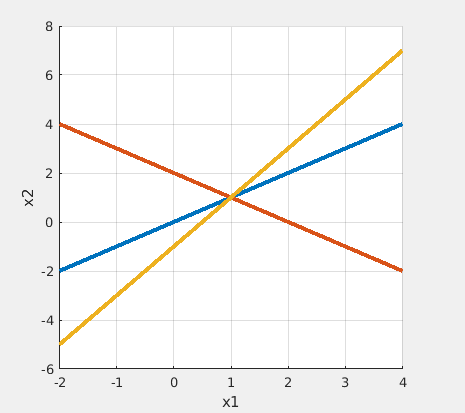
\includegraphics[scale=1]{lecture5_fig5.png} \\\\
\scalebox{2}{$-x_1+x_2=0$}\\\\
\scalebox{2}{$x_1+x_2=2$}\\\\
\scalebox{2}{$-2x_1+x_2=-1$}
\end{itemize}

\newpage
\Large
\item \textbf{ We also want our answer to have as little \scalebox{1.5}{error} as possible} \\
	\begin{itemize}
		\item \textbf{What causes error in the numerical methods?} \\
			``In software engineering and mathematics, numerical error is the combined effect of two kinds of error in a calculation. The first is caused by the finite precision of computations involving floating-point or integer values. The second usually called truncation error is the difference between the exact mathematical solution and the approximate solution obtained when simplifications are made to the mathematical equations to make them more amenable to calculation.''-wikipedia\\
		\item \textbf{2 (or 3) Major Causes} \\
			\begin{itemize}
				\item \textbf{floating point computations} \vspace{20mm}\\
				\item \textbf{truncation and solution simplification} \vspace{20mm}\\
				\item \textbf{system condition} \vspace{20mm}\\
			\end{itemize}
	\end{itemize}

\newpage
\item \textbf{ The {\B System Condition} can cause problems!} \\
\begin{itemize}
	\item An {\PR ill-conditioned} system can cause error. \\\\
	
	\item A system is {\PR ill-conditioned} if small changes in the coefficients on the either side of the equation create large variations in the solution.\\\\

	\item Let us look at a simple 2x2 example. \\\\
	
		\scalebox{1.5}{$x_1 - x_2=5$} \\\\
		\scalebox{1.5}{$kx_1 - x_2=4$}\\\\
	
	\item The system shown will have huge variations in the solution if \scalebox{1.5}{$k\approx 1$}\\\\
	
		\scalebox{1.5}{$x_1 - x_2=5$} \\\\
		\scalebox{1.5}{$(0.99)x_1 - x_2=4$}\\\\
	\item When \scalebox{1.5}{$k = 0.99$}, this gives a solution \scalebox{1.5}{$(x_1,x_2)=(100, 95)$}	\\\\
	
	\scalebox{1.5}{$x_1 - x_2=5$} \\\\
		\scalebox{1.5}{$(1.01)x_1 - x_2=4$}\\\\
	\item When \scalebox{1.5}{$k = 1.01$}, this gives a solution \scalebox{1.5}{$(x_1,x_2)=(-100, 105)$}	

\end{itemize}
\newpage 

	 \item \textbf{ \LARGE REMINDER - Homework 3 is posted and is due next Friday !} \\
 \item \textbf{ \LARGE REMINDER -Exam1 is coming up!} \\
\end{itemize}


	

\end{document}



